 %&latex
\documentclass[smaller,a4paper,allowframebreaks]{beamer}
\usepackage{amsmath,amssymb,pdfsync,listings}
\usepackage{verbatim}
\usepackage{graphicx}
\usepackage{truncate}
\usepackage[final]{pdfpages}
\usepackage{times}
\usepackage{pgffor}
\usepackage{listings}
\usepackage[english]{babel}

\begin{document}
\title{Computing Derivatives}
\frame{\titlepage}

\begin{frame}
\frametitle{Three Methods For Computing Derivatives}
Assume we want to implement the Newton method like in the previous exercise
but we don't want to require the user to pass the formula for the derivative.

Our code will need to compute the derivative internally. 
There are three main approaches for computing derivatives:

\begin{description}
\item [Numerical Differentiation] Substitute the derivative with an increment ratio, eg.
$$
f^{\prime} \simeq \dfrac{f(x+h) - f(x-h)}{2h}
$$
\item [Symbolic Differentiation] Manipulate the symbolic expression following the rules of calculus and compute the formula for the derivative.
\item [Automatic Differentiation] Is a set of techniques to numerically evaluate the derivative of a function specified by a computer program.
\end{description}
\end{frame}


\begin{frame}
\frametitle{Exercise 1}

\begin{itemize}
\item Reimplement the newton class of the previous exercise using centered finite differences to compute the derivative internally
      \begin{itemize}
            \item Add a publuic method to compute the derivative
      \item Test the convergence on the same problem as the previous exercise
      \item Study the accuracy of the derivative as a function of the increment $h$
      \end{itemize}      
\end{itemize}
\end{frame}

\begin{frame}
\frametitle{Exercise 2}

\begin{itemize}
\item Reimplement the newton class of the previous exercise using automatic differentiation to compute the derivative internally
      \begin{itemize}
      \item Test the convergence on the same problem as the previous exercise
      \item Study the accuracy of the derivative as a function of the increment $h$
      \end{itemize}      
\end{itemize}
\end{frame}

\begin{frame}
\frametitle{About Automatic Differentiation}

One of the most common algorithms for Automatic Differentiation is \textbf{Forward Accumulation}

In forward accumulation AD, one first fixes the independent variable to which differentiation is performed and computes the derivative of each sub-expression recursively. In a pen-and-paper calculation, one can do so by repeatedly substituting the derivative of the inner functions in the chain rule:

\center{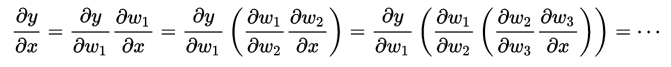
\includegraphics[width=.7\linewidth]{./images/formula_1.png}}

\end{frame}

\begin{frame}[fragile,allowframebreaks]
\frametitle{Implementation of Automatic Differentiation in C++}

\begin{lstlisting}[language=C++]
class
var
{
  std::function<double (double)> val;
  std::function<double (double)> der; 

public:

  var ()
    : val ([] (double x) -> double { return x; }),
      der ([] (double x) -> double { return 1.0; })
  { };

  var (std::function<double (double)> val_,
       std::function<double (double)> der_)
    : val (val_), der (der_)
  { };
\end{lstlisting}

\begin{lstlisting}[language=C++]
  double
  eval (double x) const
  { return val (x); };

  double
  eval_der (double x) const
  { return der (x); };  
};
\end{lstlisting}

\begin{lstlisting}[language=C++]
var sin (var X);
var cos (var X);
var exp (var X);

var operator* (double a, var X);
var operator* (var X, double a);
var operator* (var Y, var X);

\end{lstlisting}
\end{frame}

\end{document}